\documentclass[11pt,onecolumn]{article}

\usepackage[lmargin=0.75in,rmargin=0.75in,tmargin=.75in,bmargin=0.7in]{geometry}


\usepackage[tbtags]{amsmath}
\usepackage{amsfonts}
\usepackage{amssymb}
\usepackage{amsthm}
\usepackage{subfigure}
\usepackage{cite}
\usepackage{calc}
\usepackage{color}
\usepackage{epsfig}
%\usepackage{setspace}
\usepackage{hyperref}
\usepackage{enumerate}
\usepackage{bm}
\usepackage{algorithmicx}
\usepackage{algpseudocode}
\usepackage{algorithm}
% \usepackage{cite}

\usepackage{caption}

\newtheorem{defn}{Definition}
\newtheorem{thm}{Theorem}[section]
\newtheorem{cor}[thm]{Corollary}
\newtheorem{prop}{Proposition}
\newtheorem{lem}[thm]{Lemma}
\newtheorem{example}{Example}
\newtheorem{conj}[thm]{Conjecture}
\newtheorem{constr}[thm]{Construction}
\newtheorem{note}{Remark}
\newcommand{\bit}{\begin{itemize}}
\newcommand{\eit}{\end{itemize}}
\newcommand{\bcor}{\begin{cor}}
\newcommand{\ecor}{\end{cor}}
\newcommand{\beq}{\begin{equation}}
\newcommand{\eeq}{\end{equation}}
\newcommand{\beqn}{\begin{equation*}}
\newcommand{\eeqn}{\end{equation*}}
\newcommand{\bea}{\begin{eqnarray}}
\newcommand{\eea}{\end{eqnarray}}
\newcommand{\bean}{\begin{eqnarray*}}
\newcommand{\eean}{\end{eqnarray*}}
\newcommand{\ben}{\begin{enumerate}}
\newcommand{\een}{\end{enumerate}}
\newcommand{\bdefn}{\begin{defn}}
\newcommand{\edefn}{\end{defn}}
\newcommand{\bnote}{\begin{note}}
\newcommand{\enote}{\end{note}}
\newcommand{\bprop}{\begin{prop}}
\newcommand{\eprop}{\end{prop}}
\newcommand{\blem}{\begin{lem}}
\newcommand{\elem}{\end{lem}}
\newcommand{\bthm}{\begin{thm}}
\newcommand{\ethm}{\end{thm}}
\newcommand{\bconj}{\begin{conj}}
\newcommand{\econj}{\end{conj}}
\newcommand{\bconstr}{\begin{constr}}
\newcommand{\econstr}{\end{constr}}
\newcommand{\bpf}{\begin{proof}}
\newcommand{\epf}{\end{proof}}
\newcommand{\bprf}{{\em Proof: }}
\newcommand{\bproof}{{\em Proof of }}
\newcommand{\eproof}{\hfill $\Box$}
\newcommand{\argmin}{\operatornamewithlimits{arg \ min}}
\newcommand{\argmax}{\operatornamewithlimits{arg \ max}}

\setlength\parindent{0pt} %noindent for all paragraphs
\algnewcommand{\And}{\textbf{and}\xspace} 
\def\today{\number\day\space\ifcase\month\or January\or February\or March\or April\or May\or June\or July\or August\or September\or October\or November\or December\fi\space\number\year} %the 'right' date format


%\pdfinfo{%
%  /Title    (HADOOP : NetApp's Perspective - Our Understanding)
%  /Author   (GK)
%  /Creator  ()
%  /Producer ()
%  /Subject  (Documentation)
%  /Keywords (Coding for Hadoop)
%}

\title{EE 377 Project Midterm Report}
\author{Govinda Kamath and Jesse Zhang}
\date{\today}


\begin{document}
\maketitle
 
\section{Background}
With recent advancements in RNA sequencing (RNA-seq) technologies, biologists have enjoyed a surplus of gene expression data at the resolution of individual cells. One of the most interesting problems in biology is that of determining the differentiation patterns of cells such as the process of a stem cell evolving (or differentiating) into a heart cell. A recent experiment [1] has produced a single-cell RNA-seq dataset consisting of 271 human primary myoblasts collected at four different times. The authors attempt to order these cells according to a so-called ``pseudotime" or a latent variable that quantifies how differentiated a given cell is. Attempts of studying cell differentiation have been performed by various groups using various methods. For example, Mueller et al. [2] attempt to order \textit{batches} of sampled cells according to the distributions of certain transcripts (or features) within clusters. For this project, we hope to combine the notion of measuring the distance between cells based on distributions of certain transcripts with the concept of ``pseudotime." We hope that by doing this, we can obtain a more biologically meaningful (and statistically sound) ordering of the 271 primary myoblasts. The success of this project could lead to meaningful insights in modeling cell differentiation; these techniques can perhaps be applied to other single-cell datasets studying the growth of cancer, for example.

\section{Problem statement}
At sampling time $t$ ($t = 1, \dots, T$), we are given $n_t$ length-$d$ vectors representing the $n_t$ cells collected at time $t$. Each cell is described with $d$ features, which can be gene expression levels, transcript expression levels, or binary markers indicating whether a particular mutation or epigenetic marker was observed. We assume that each data is some mixture of two or more populations (or cell types). In other words, each point (cell) lived somewhere on a continuum \textit{between} cell types before being sampled (collected). The goal is to learn something about the structure of this continuum. \\

As stated in our project proposal, one potential approach taken in [3] is to cluster the $N = \sum_{t} n_t$ cells into $k$ clusters and then draw a minimum-spanning tree (MST) through the $k$ centroids. In this case, the MST supposedly captures the underlying structure. We feel that a more intuitive model is a continuous-time Markov chain (CTMC) where states represent cell types and transition rates represent times required to transition from one cell state to another. After assigning a probability density to each state, we would want to do inference on such a model. One reason for choosing the CTMC is that it's easier to analyze statistically than arbitrary clustering algorithms. 
 

\section{Preliminary results}
We quickly realized that there were several layers of complexity to this problem even with the CTMC assumption. For real-life datasets, one may not necessarily know $K$, the number of states, $\{\lambda_i\}_{i=1}^M$, the exponential rate parameters associated with the $M$ edges, $p_S(x)$, the noise model associated with each state (i.e. how observations of cells in state $S$ are distributed), or even which of the $K \choose 2$ pairs of states should have edges connecting them. \\

As a first step, we assume that we know the underlying structure of the CTMC. Inspired by the results from [1], we assume that samples come from one of 4 cell types described by the CTMC in Figure 1. In the case of [1], state $A$ would be a proliferating cell, state $C$ would be a differentiating myoblast, state $D$ would be an interstitial mesenchymal cell, and state $B$ would be some intermediate hybrid of the first 3 states. Another key assumption we make here is that we can look at the same cell multiple times (or once at each observation time).

\begin{figure*}[!htb]
		\captionsetup{width=.8\linewidth}
		\caption{Assumed underlying structure for preliminary results. Here, cells start in state $A$. After spending $t_A \sim \textsf{Exp}(\lambda_1) $ in state $A$, a cell transitions to an intermediate state $B$ before ending as either a type $C$ cell or a type $D$ cell. After arriving at state $B$, the end state of this particular cell is determined by the outcome of an exponential race between $\lambda_2$ and $\lambda_3$.}
		\centering
		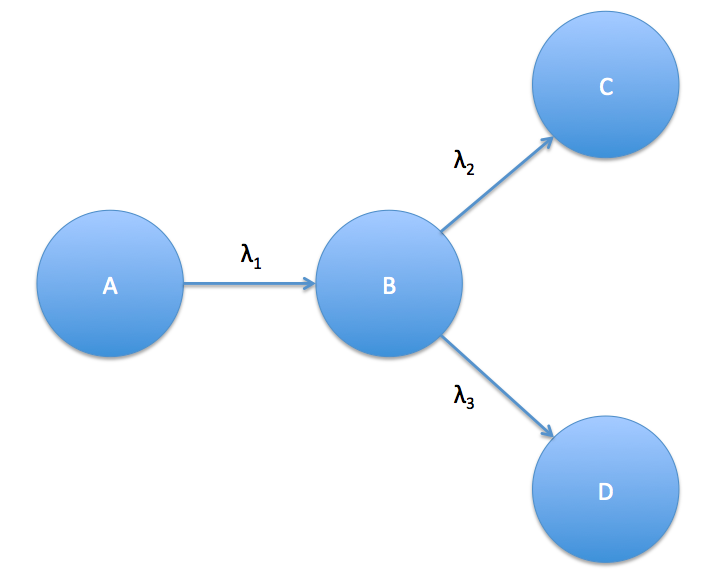
\includegraphics[scale=0.3]{Fig1.png}
\end{figure*}

Given this CTMC, we can simulate data by setting the number of samples, the values of $\lambda_1, \lambda_2, \lambda_3$, and the observation times, as shown in Figure 2. Using $\lambda_1 = 0.5, \lambda_2 = 1, \lambda_3 = 0.25$, we generate 100 samples. All 100 samples start as cell type $A$.

\begin{figure*}[!htb]
		\captionsetup{width=.8\linewidth}
		\caption{Simulation using the CTMC from Figure 1. 200 cells are sampled and tracked at 5 observation times. We see that as the observation time increases, cells evolve from type $A$ to ultimately type $C$ or $D$.}
		\centering
		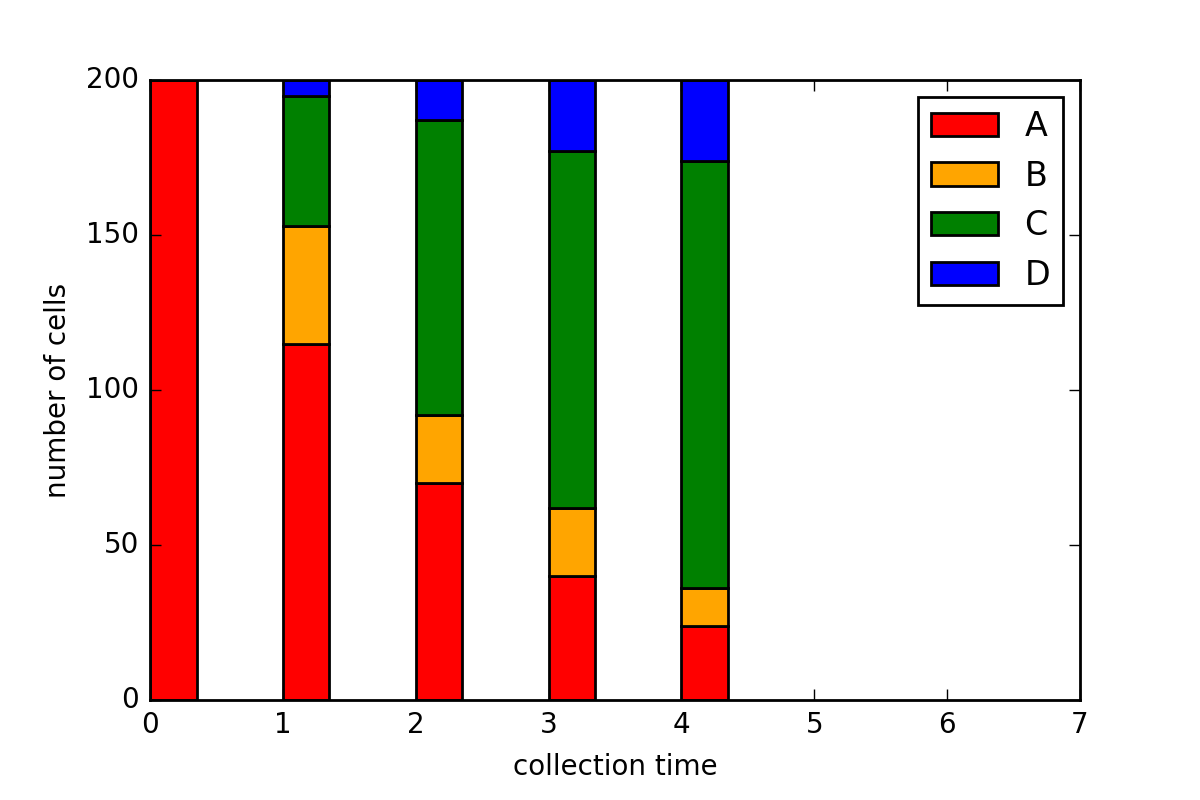
\includegraphics[scale=0.65]{Fig2.png}
\end{figure*}

Given the structure of the CTMC and these observations, we can easily estimate both all rate parameters. Let $P_t(S_1,S_2)$ represent the probability of going from state $S_1$ to state $S_2$ after $t$ time has passed, and let $t_S$ represent the amount of time a cell spends in state $S$. Then
\begin{align*}
	P_t(A,A) = P(t_A \geq T) = e^{-\lambda_1 t} \implies \hat{\lambda}_1 = -\frac{1}{t} \log \frac{\# \mbox{ type $A$ cells at $t$}}{\# \mbox{ type $A$ cells at time 0}}
\end{align*}
After estimating $\lambda_1$, we can estimate $\lambda_2$ and $\lambda_3$ using a slightly more complicated derivation:
\begin{align*}
	P_t(A,B) & = \int_0^t P(t_A) P(t_B \geq t_1 - t_A) dt_A \\
	& = \int_0^t \lambda_1 e^{-\lambda_1 t_A} (e^{-(\lambda_2+\lambda_3)(t-t_A})dt_A \\
	& = \frac{\lambda_1 e^{(\lambda_2+\lambda_3)t}}{-\lambda_1+\lambda_2 + \lambda_3} \left(e^{t(-\lambda_1 + \lambda_2 + \lambda_3)}-1 \right)
\end{align*}
Using $\hat{\lambda}_1$ and the ratio of number of $B$ cells at time $t$ to the number of $A$ cells at time 0, we can estimate $\lambda_2 + \lambda_3$. Additionally, we know the ratio of $\lambda_2$ to $\lambda_3$ from the observations. We solve a system of equations to obtain estimates for $\lambda_2$ and $\lambda_3$. This approach seems to work reasonably well, and for the example from Figure 2 we obtain rate parameter estimates of $\hat{\lambda}_1 = 0.54, \hat{\lambda}_2 = 1.11,$ and $\hat{\lambda}_3 = 0.25$. \\

Next we simulate noisy observations of each cell at each observation time. We assume that given states $S = \{A,B,C,D\}$ and $K = |S|$, observations are distributed $p_S(x) = \textsf{N}(\mu_i,\sigma^2 I_K)$ where $\mu_i \in \mathbb{R}^K$. Using the states shown in Figure 2, we simulate observations at each of the five times by setting $\mu_A = (0,0), \mu_B = (1,0), \mu_C = (2,1), \mu_D = (2,-1)$, and $\sigma^2 = 0.05$. The results of the simulation are presented in Figure 3.

\begin{figure*}[!htb]
		\captionsetup{width=.8\linewidth}
		\caption{Noisy observations are simulated from the cells of Figure 2, resulting in 200 noisy samples at each observation time. We see that the cells shift from the left (states $A$ and $B$) to the right (end states $C$ and $D$) as time increases.}
		\centering
		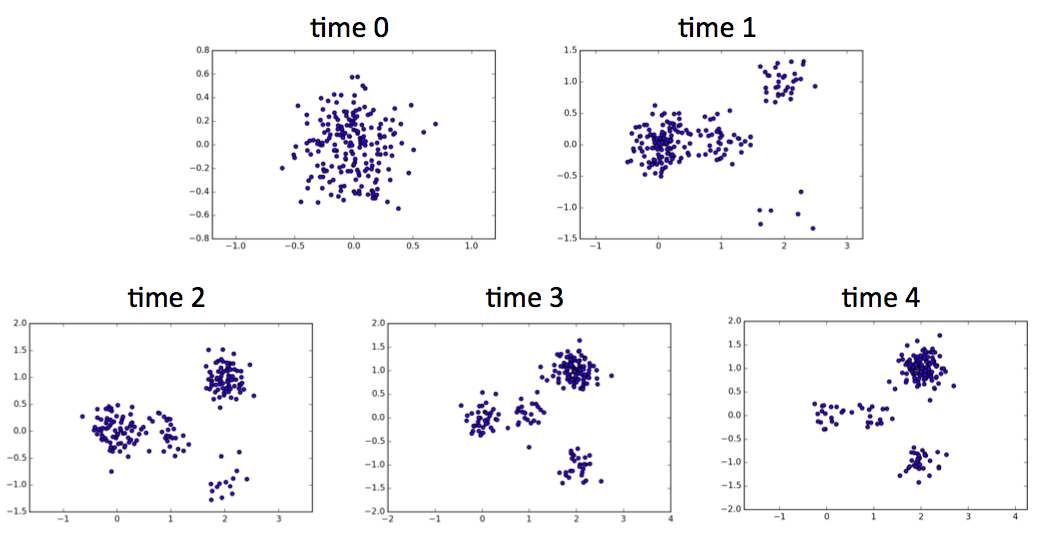
\includegraphics[scale=0.35]{Fig3.png}
\end{figure*}

Because we know both the number of clusters and that the observations are distributed iid Gaussian, at each observation time we can infer the states of the observed cells using a mixture of Gaussians model, which can be easily solved with a standard expectation-maximization (EM) algorithm. We use the Hungarian algorithm to match the labels output by EM with the true labels, resulting in the cluster assignments shown in Figure 4. \\

\begin{figure*}[!htb]
		\captionsetup{width=.8\linewidth}
		\caption{Cluster assignments of each observation generated in Figure 3 using EM.}
		\centering
		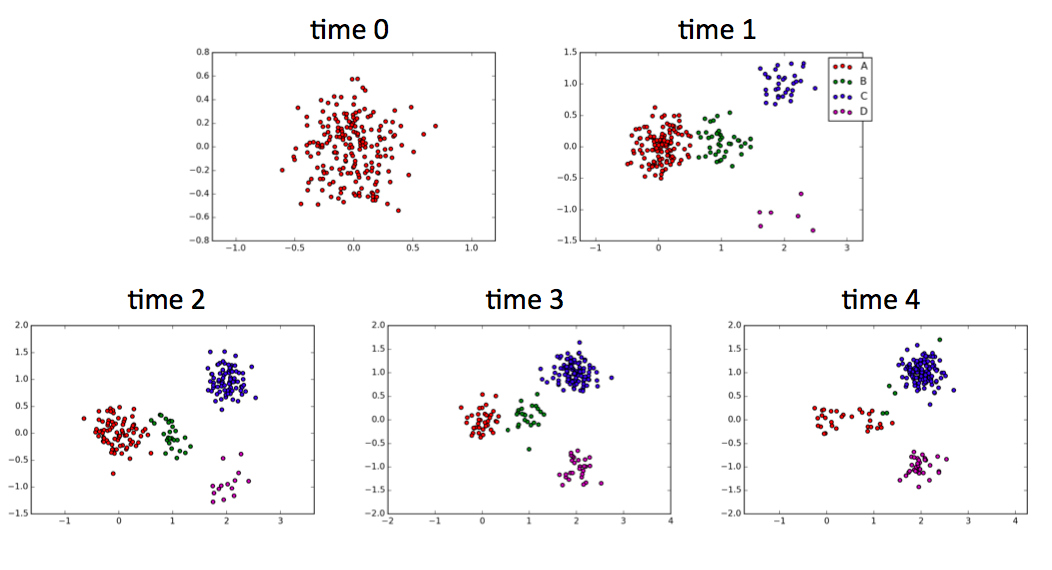
\includegraphics[scale=0.35]{Fig4.png}
\end{figure*}

After assigning points to states, we can estimate the exponential rates just as before: $\hat{\lambda}_1 = 0.49, \hat{\lambda}_2 = 1.29,$ and $\hat{\lambda}_3 = 0.27$. While the estimates are on average a bit worse, we still seem to do reasonably well.

\section{Next steps}
Initial simulations seem to generate promising results because we have made several strong simplifying assumptions. In the case of the dataset presented by [1], individual data points are high-dimensional vectors (length 47192), making EM much more difficult to compute. Determining the correct method for reducing the dimensionality of the data proves to be a challenge. Additionally, we have no reason to believe that observations come from one of $K$ Gaussian distributions. We have no reason to believe that the Gaussian, equal-variance, or independence assumptions are true. In fact, we intuitively expect the evolution of a cell to be a gradual process, and therefore $\mu$ should be a function of some latent time variable. Finally, the set of cells sampled using real data is completely different at each observation time. Ideally, we would be able to account for the the fact that we do not observe time 0 as the first observation does not show a homogenous population of cells all of one type. \\

If our model is correct, we would like to say something about the guarantees we can make as a function of the CTMC complexity (number of nodes and edges), the number of samples, and the number of observation time.

\section{References}
\begin{enumerate}
	\item Trapnell, Cole, Davide Cacchiarelli, Jonna Grimsby, Prapti Pokharel, Shuqiang Li, Michael Morse, Niall J. Lennon, Kenneth J. Livak, Tarjei S. Mikkelsen, and John L. Rinn. "The dynamics and regulators of cell fate decisions are revealed by pseudotemporal ordering of single cells." Nature biotechnology 32, no. 4 (2014): 381-386.
	\item Mueller, Jonas, Tommi Jaakkola, and David Gifford. "Modeling Trends in Distributions." arXiv preprint arXiv:1511.04486 (2015).
	\item Ntranos, Vasilis, Govinda M. Kamath, Jesse Zhang, Lior Pachter, and N. Tse David. "Fast and accurate single-cell RNA-Seq analysis by clustering of transcript-compatibility counts." bioRxiv (2016): 036863.
\end{enumerate}

\end{document}
